\begin{refsection}
    \chapter{Further investigations into Ch-bonding at oxygen.}
    \label{app:o-ch-bonding}
    
    \section{Introduction}
    Following our initial discovery of unconventional Ch-bonding in \emph{o}-nitro-O-aryl oximes, we sought to establish a structural correlation to bring it in line with more typical Ch-bonding.
    To this end, we attempted to manipulate the electron density on both Ch-bond donor and acceptor, and measure the structural changes that result.
    We believed that this was important to further substantiate our claim of Ch-bonding being a significant stablising factor.
    
    \section{Results and discussion}
    
    \subsection{CSD search}
    Since the publication of our first report, we became aware of other apparent Ch-bonds involving oxygen, although they were not initially recognised as such.
    Consistent with expectations, they both involve oxygen atoms bonded to nitrogen.
    The packing of bis-furoxan \textbf{XERPOA} is directed by intermolecular \ce{O\cdots O} Ch-bonds, although the structure is also stablised by the \ce{Rb+} counterion (not shown).\autocite{Gilardi2005}
    The classic oxaziridine electrophilic oxygen species \textbf{FIVJEZ} also exhibits a Ch-bond between the oxygen and the chlorine on an adjacent molecule.\autocite{Malpezzi1987}
    Both structures are shown in figure \cref{fig:furoxan-oxaziridine}.
    The presence of these \emph{inter}molecular Ch-bonds is encouraging, as it indicates that oxygen-based Ch-bonds are competitive with other interactions, and therefore likely to be of interest for the purposes of drug discovery or crystal engineering.\autocite{Taylor2020IdentifyingCompetitive}
    
    \begin{figure}
        \centering
        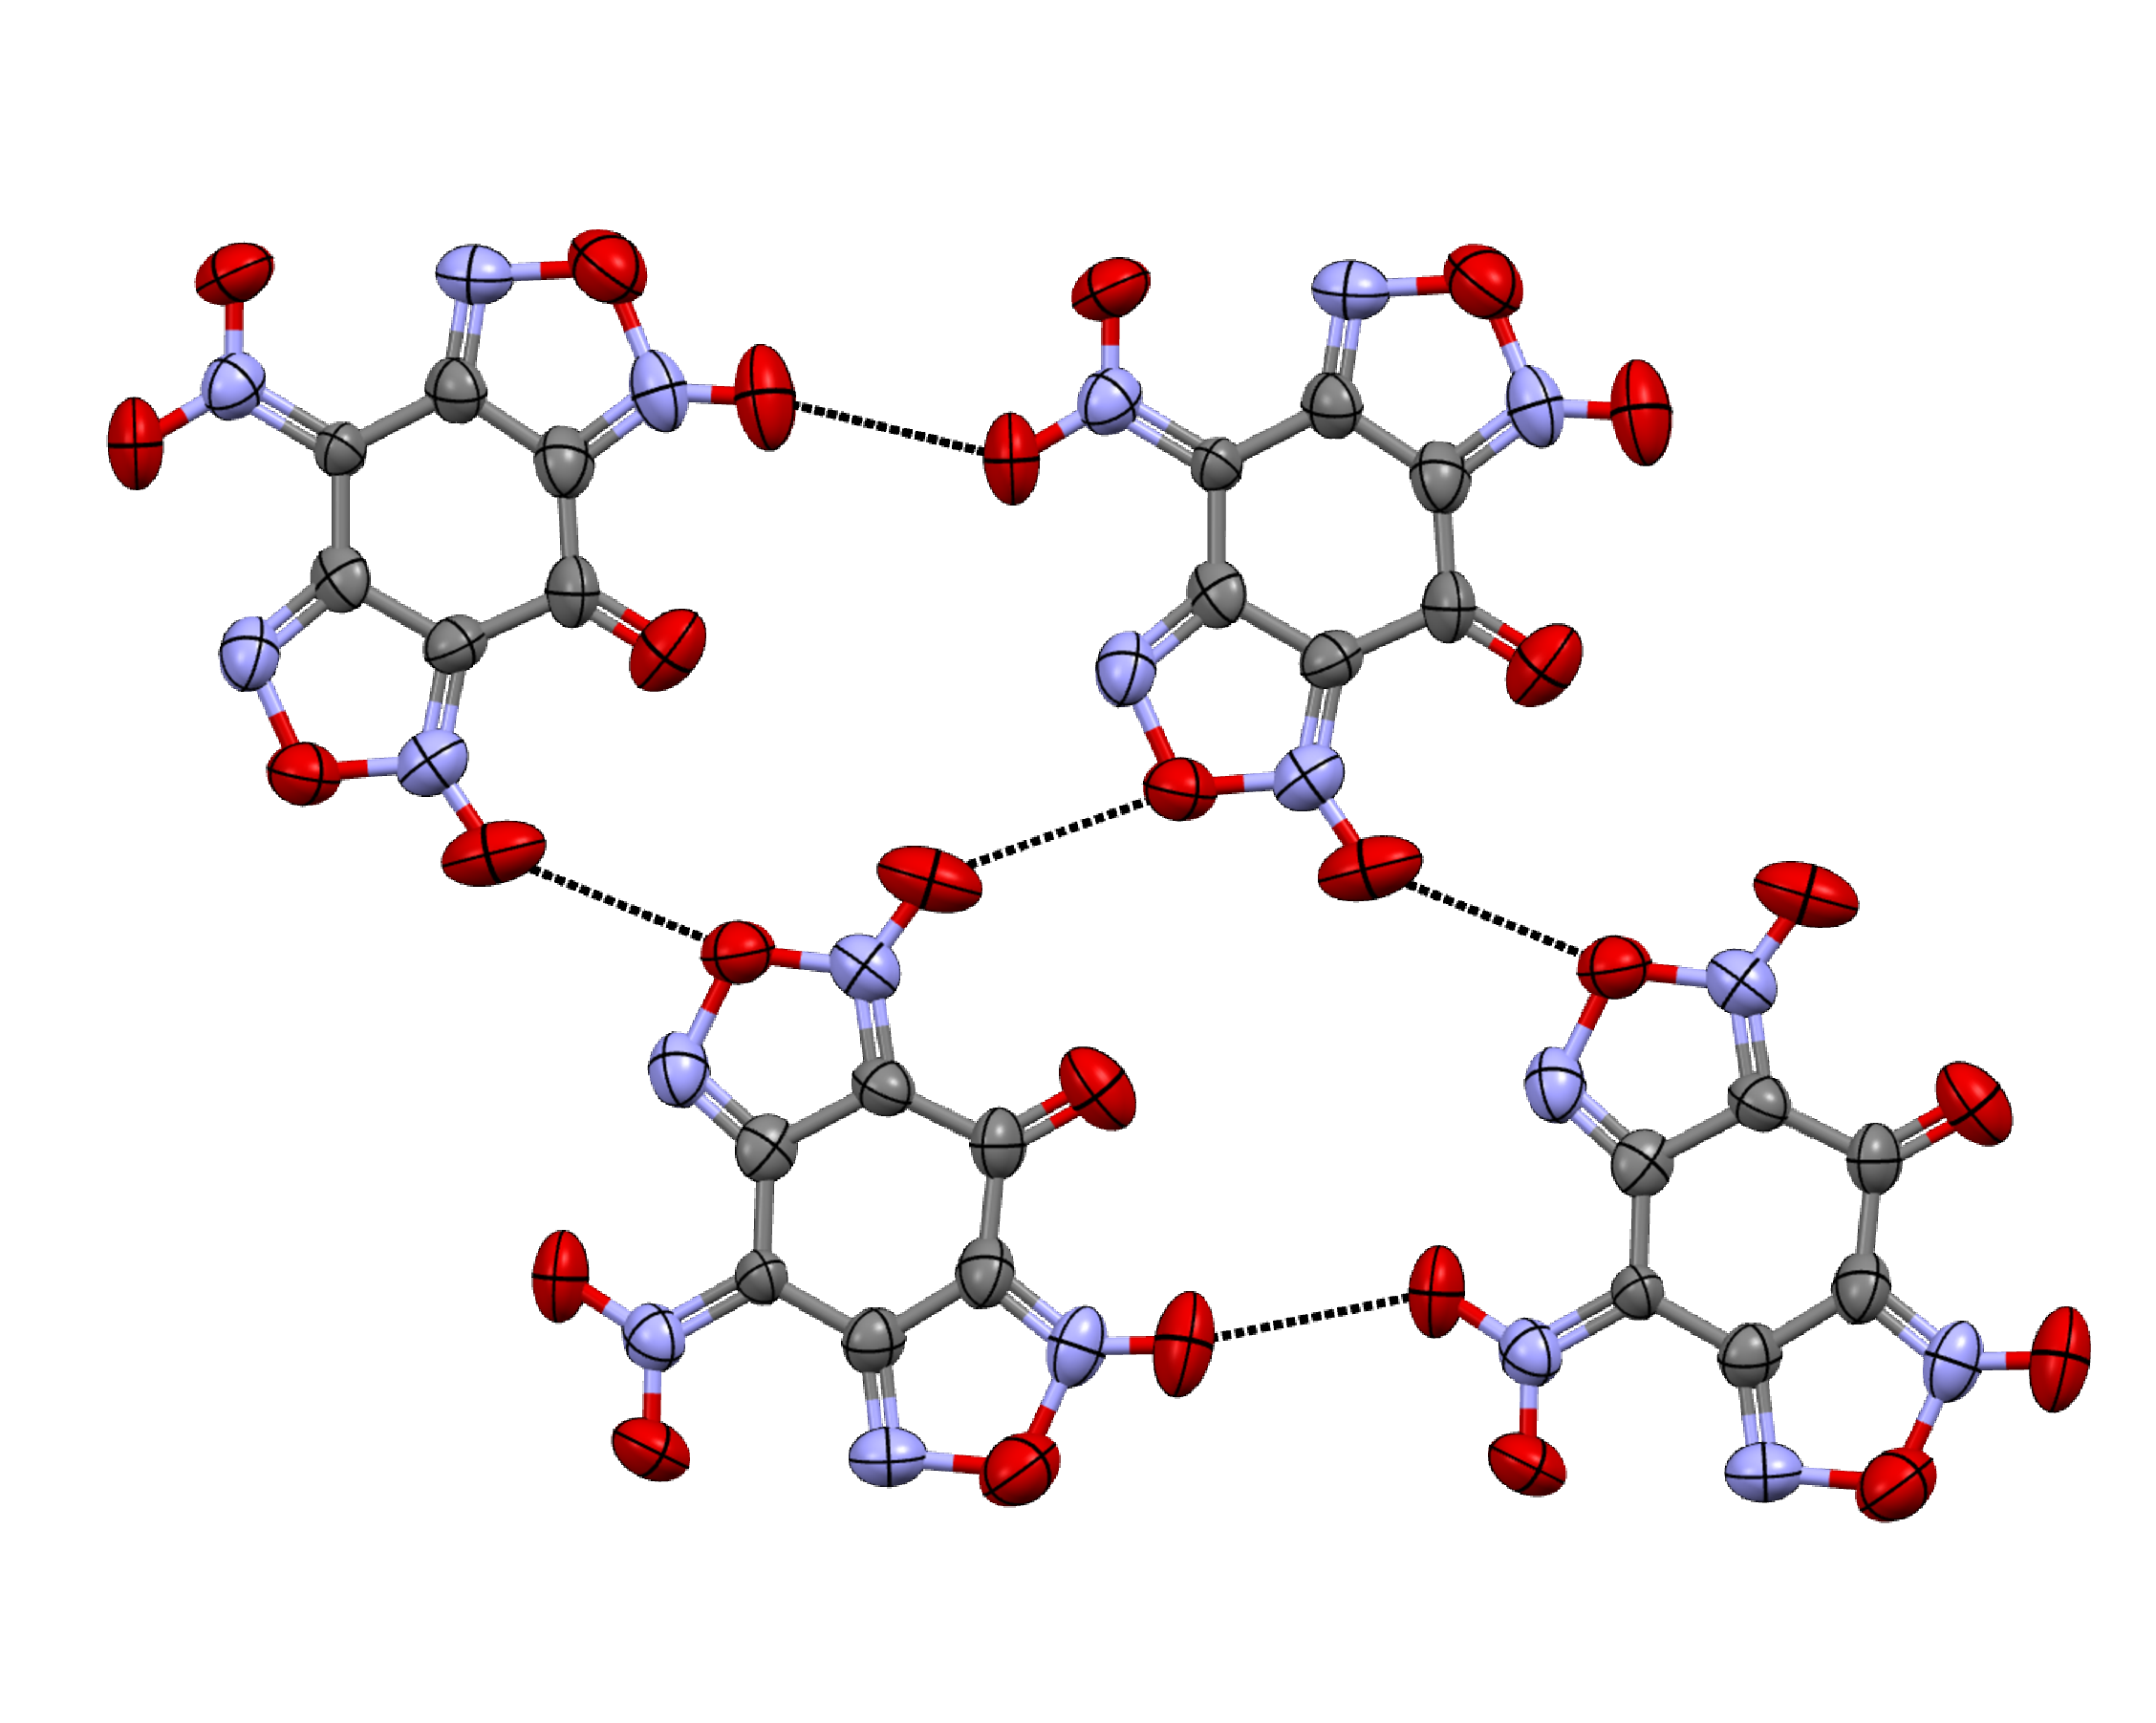
\includegraphics[width=0.45\textwidth]{Figures/XERPOA.pdf}
        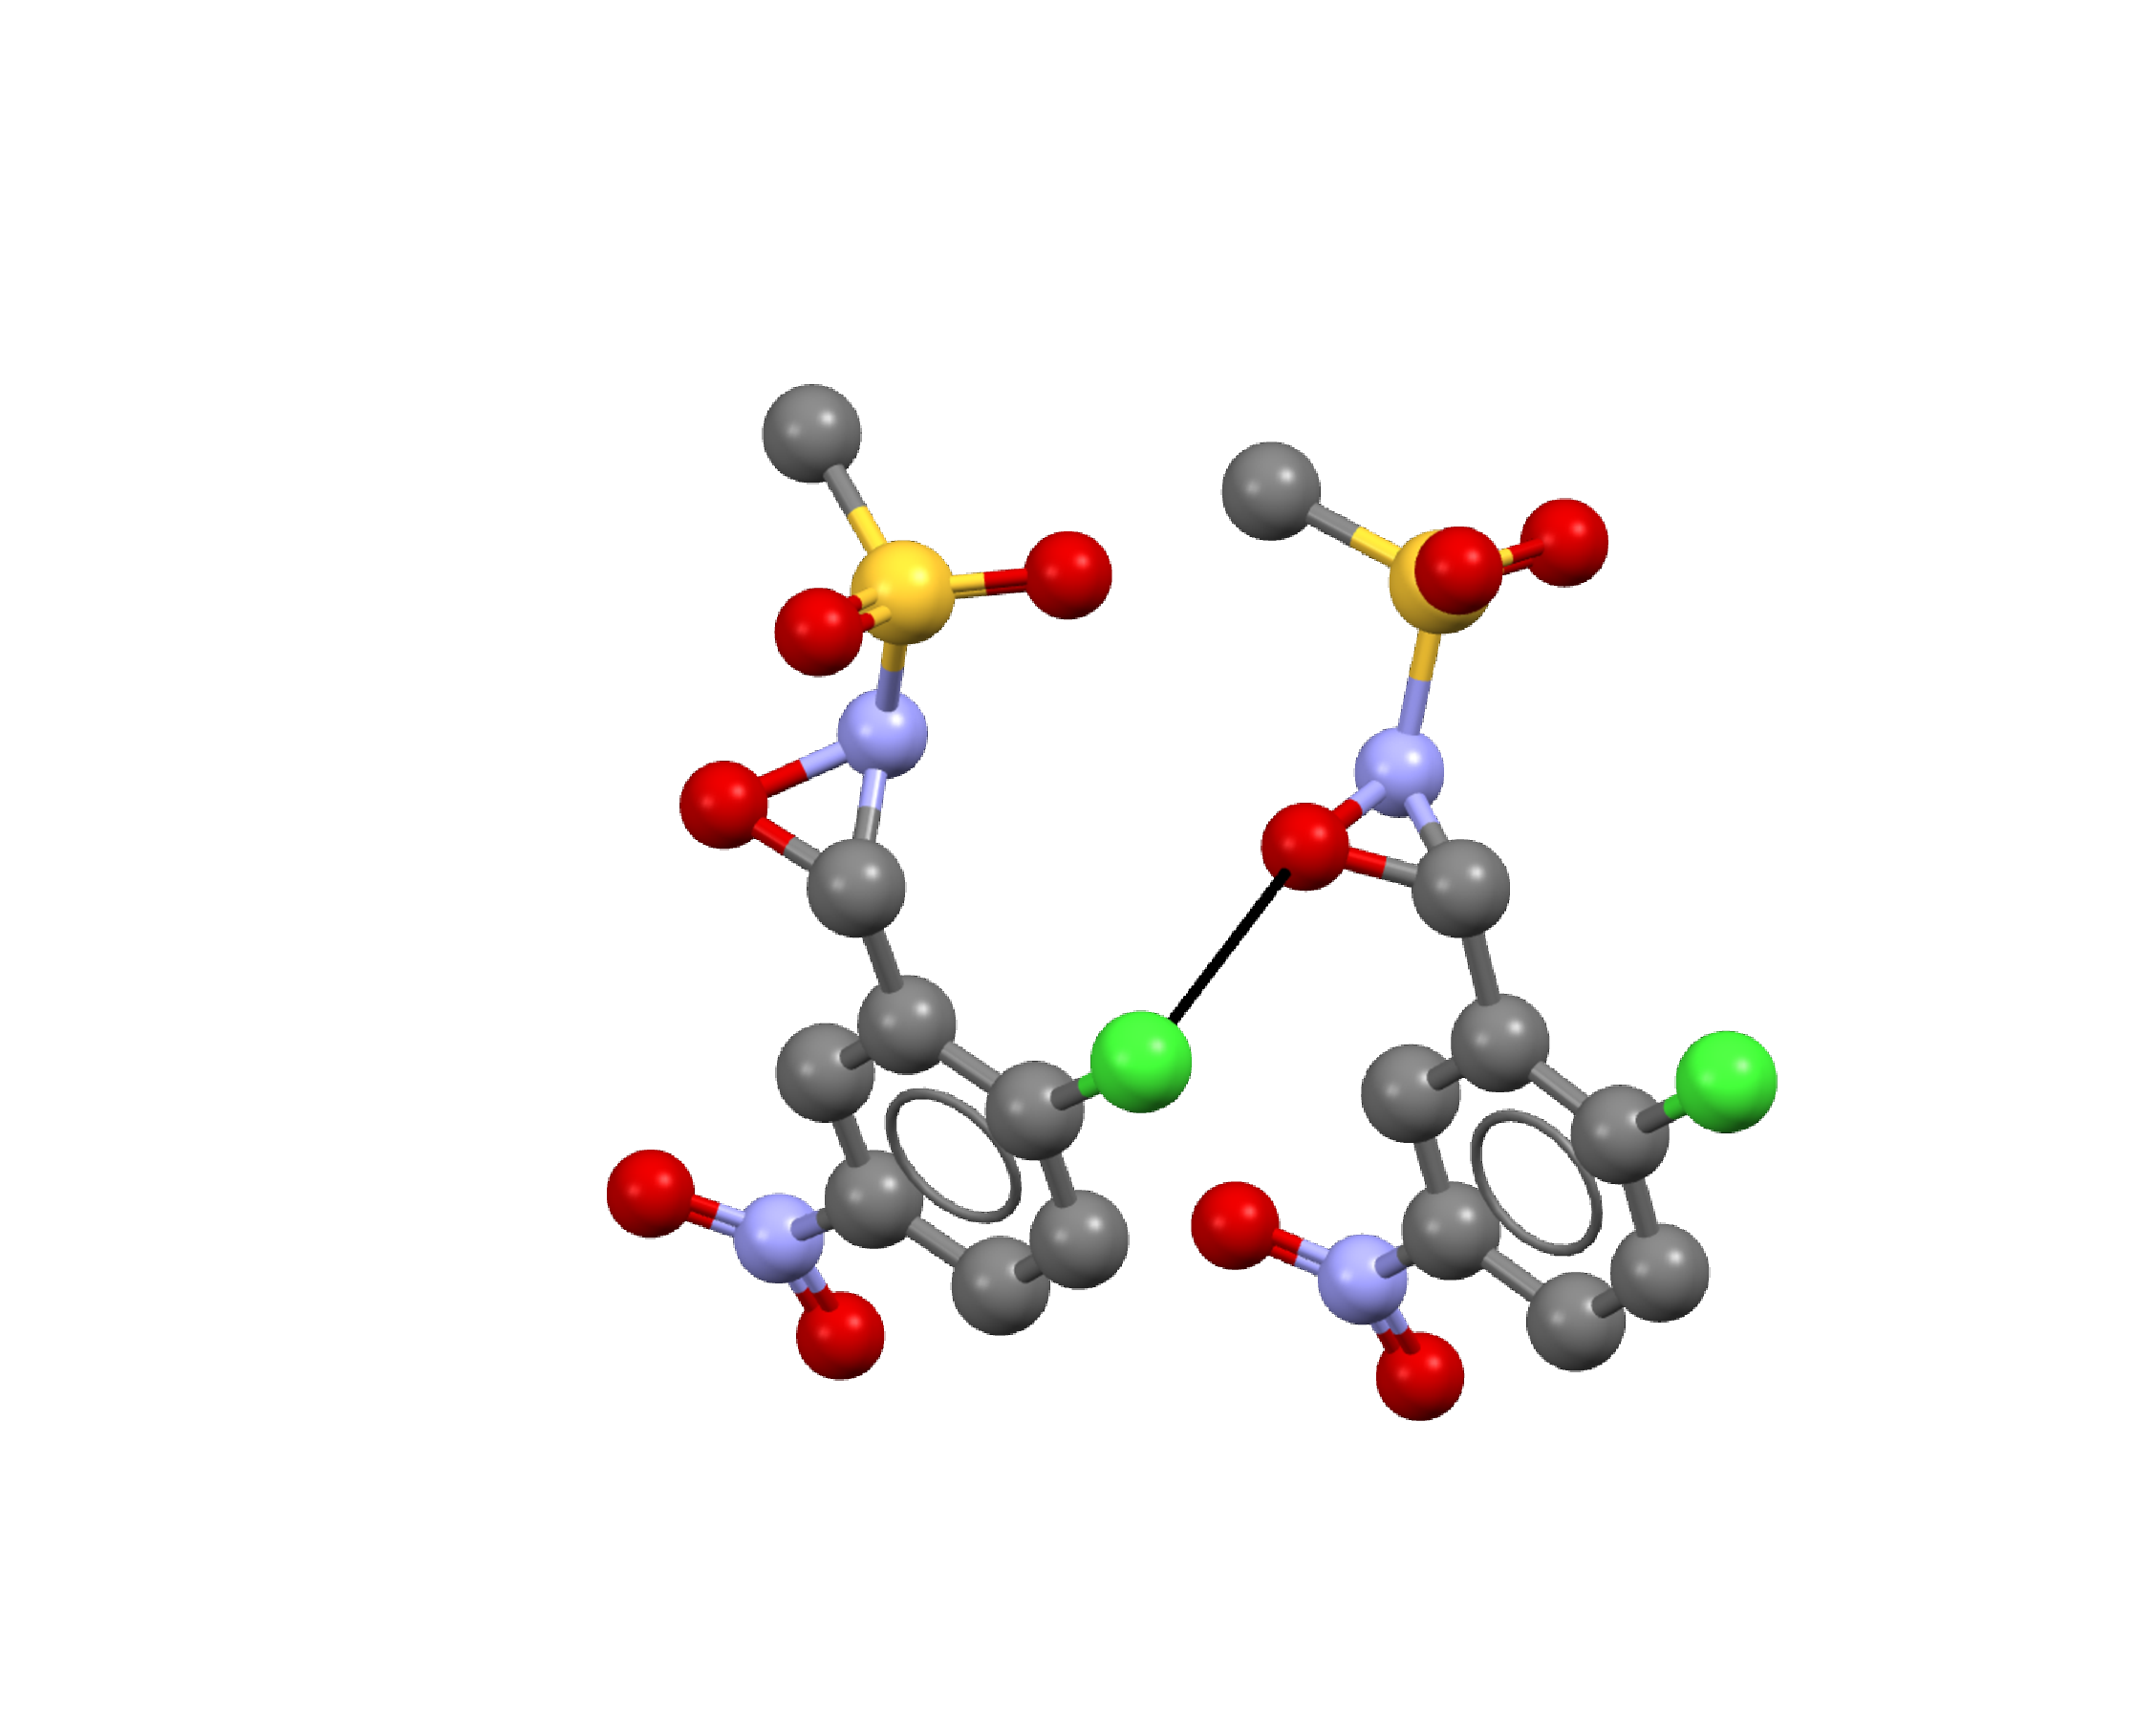
\includegraphics[width=0.45\textwidth]{Figures/FIVJEZ.pdf}
        \caption{Structures of \textbf{XERPOA} and \textbf{FIVJEZ} with Ch-bonds indicated by black dotted lines.}
        \label{fig:furoxan-oxaziridine}
    \end{figure}
    
    \subsection{Structural studies of analogues}
    As the Ch-bond appears to be a primarily electrostatic interaction, it follows that the strength of the Ch-bond will be correlated with the difference in electrostatic potential between the donor and acceptor.
    
    To test this, we synthesised a series of analogues which varied in the electron density at the nitro and oxime groups.
    We first attempted to investigate the effects of substantially increasing the electrophilic character of the oxime oxygen, by starting from an electron-poor oxime.
    Initial efforts to form hexafluoroacetone oxime (from hexafluoroaceteone deuterate and hydroxylamine) were hampered by the fact that the dehydration equilibrium strongly favours the hemiaminal form (figure \cref{sch:hexafluoroacetone}).
    
    \begin{figure}
    \centering
    \begin{subfigure}{0.5\linewidth}
        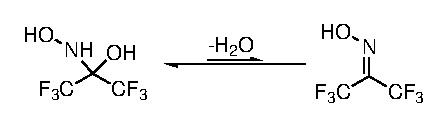
\includegraphics[scale=0.74,trim=0 -1cm 0 -1cm]{Figures/hexafluoroacetone.eps}
    \end{subfigure}
    \begin{subfigure}{0.5\linewidth}
        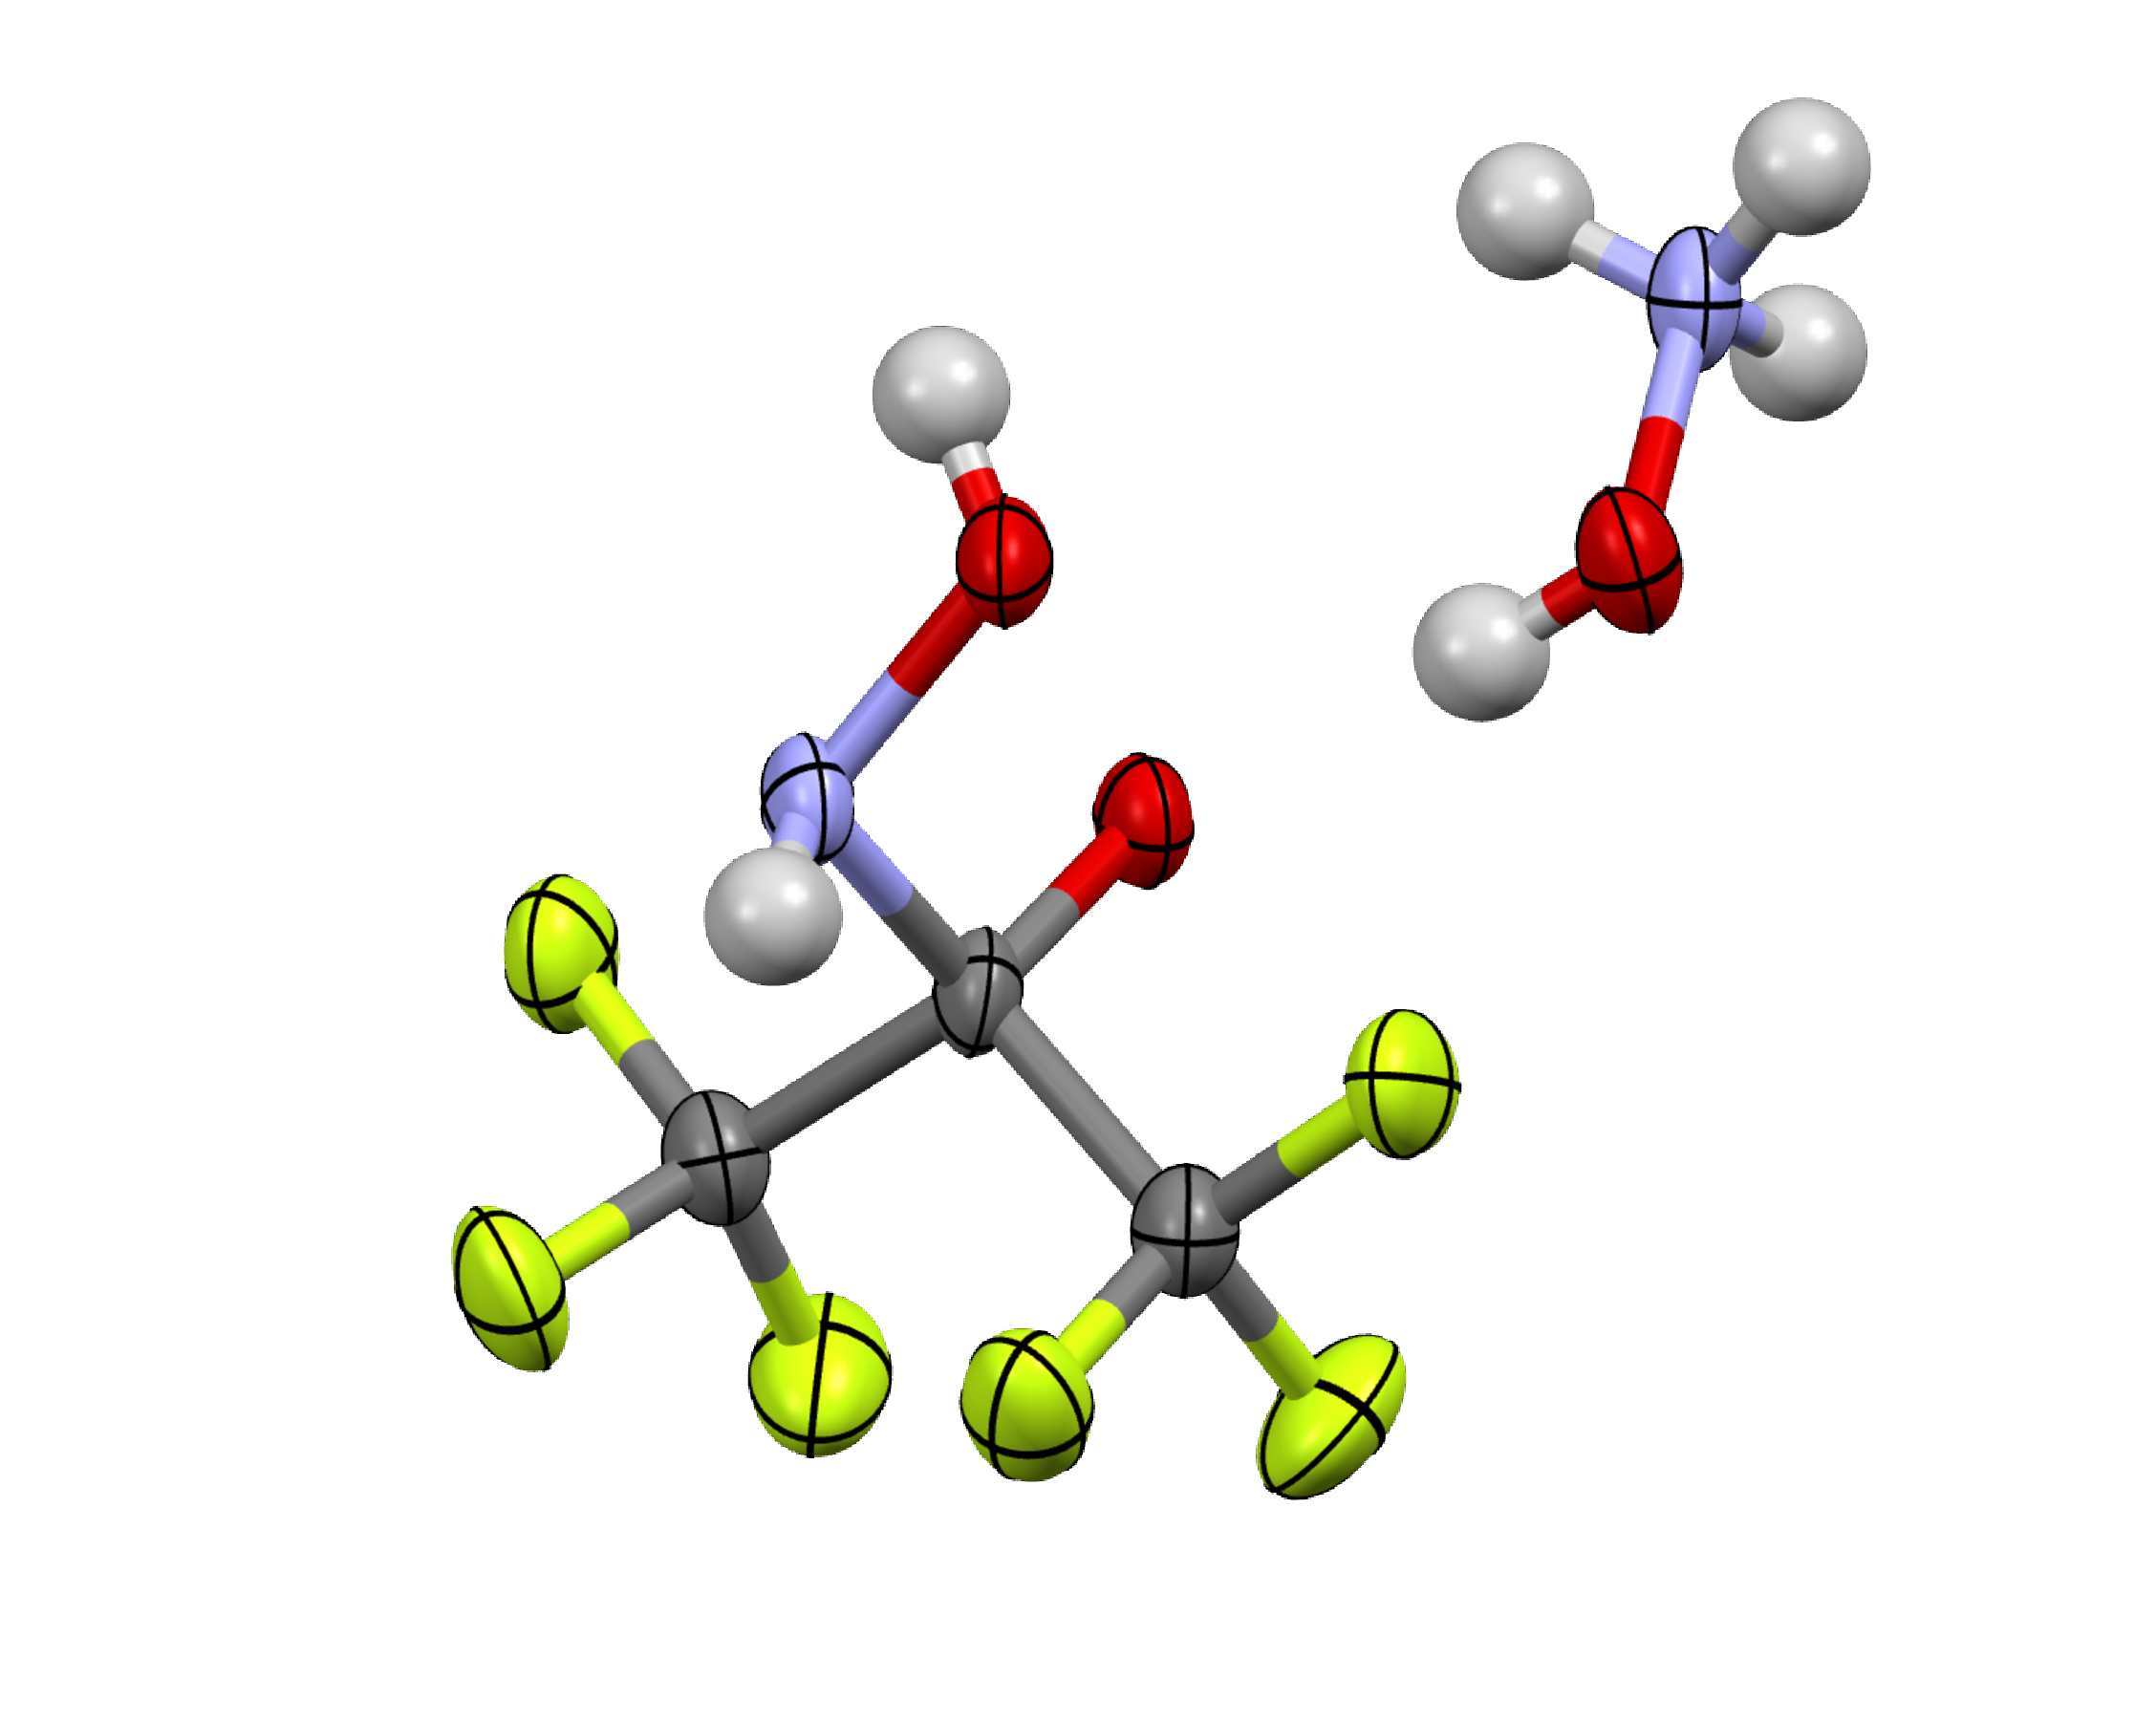
\includegraphics[width=4cm]{Figures/hexafluoroacetone_oxime.pdf}
    \end{subfigure}
    \caption[Dehydration of electron poor hemiaminals]{The dehydration of electron poor hemiaminals is strongly disfavoured. Instead, the hydroxylammonium salt was isolated as a crystalline solid.}
    \label{sch:hexafluoroacetone}
    \end{figure}
    
    Various methods to remove the water failed, so we persisted with the cyclohexanone oxime (as these derivatives had been shown to crystallise well) and instead modified the electronic properties of the aryl group.
    
    We first prepared the derivative lacking a nitro group at the 4 position of the aryl ring (compound \cmpd{cyclohexanone-oxime-2np}).
    Removing the electron-withdrawing nitro group at this position make the oxime oxygen somewhat more electron rich, while having a negligible effect on the Lewis basicity of the other nitro group.
    This has the effect of "switching off" the Ch-bond, by reducing its strength relative to other effects.
    Indeed, this can be observed in the crystal structure (figure \cref{fig:cyclohexanone-oxime-2np}), where the nitro group adopts a twisted orientation similar to that of \cmpd{acetone-oxime-dnp}.
    
    \begin{figure}
    \centering
    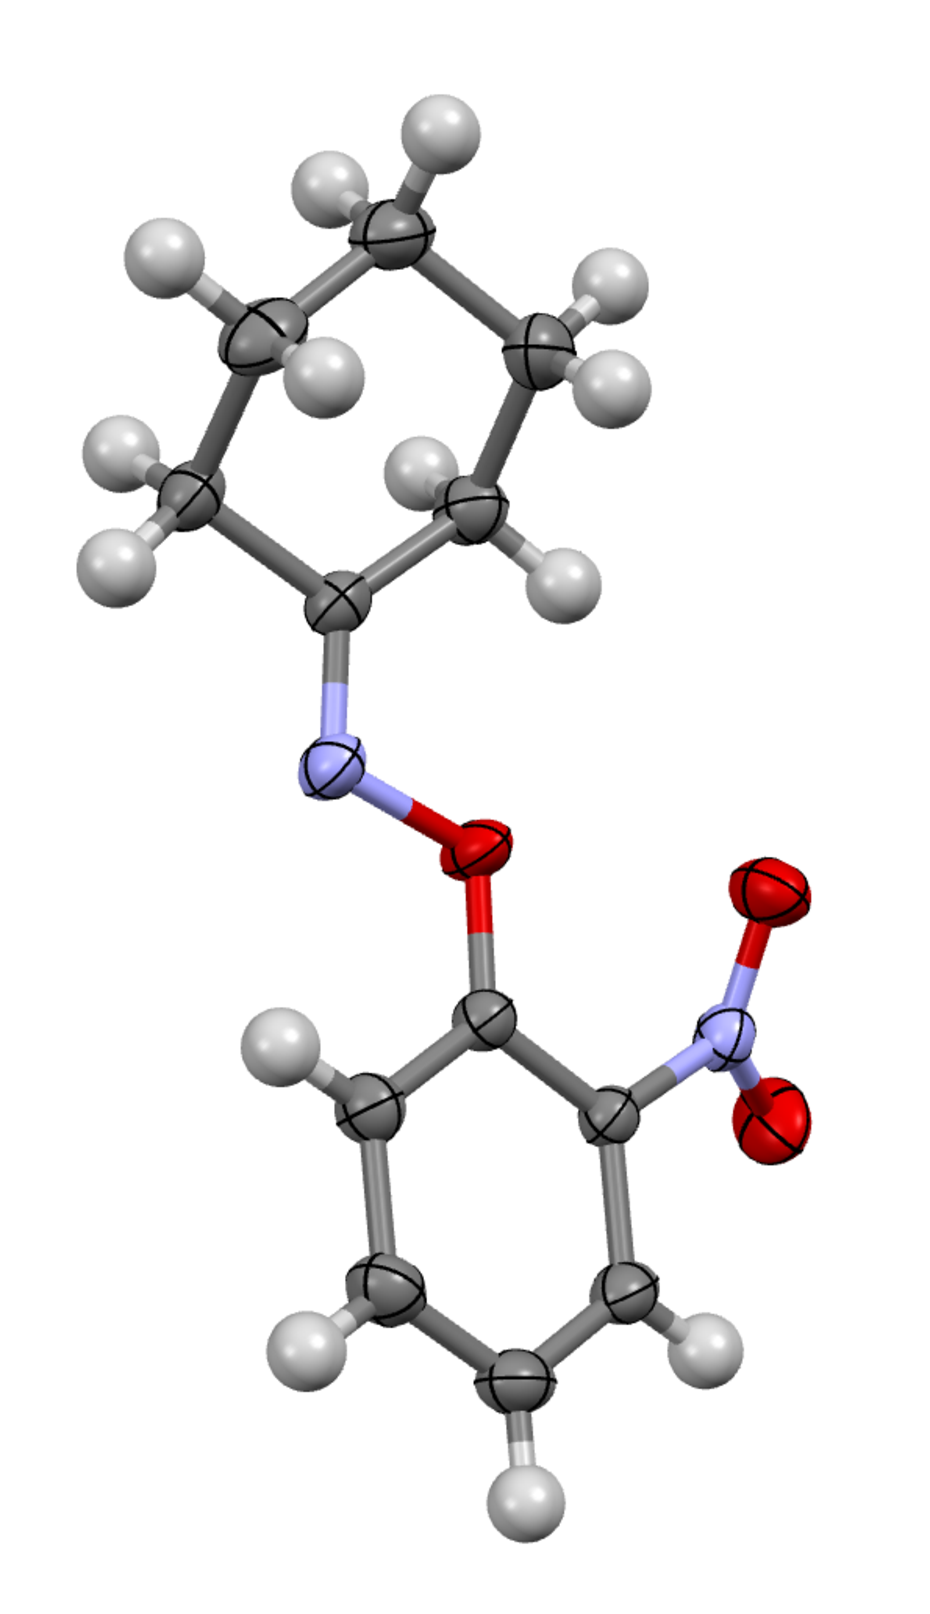
\includegraphics[height=4cm]{Figures/cyclohexanone-oxime-2np.pdf}
    \replacecmpd{cyclohexanone-oxime-2np}
    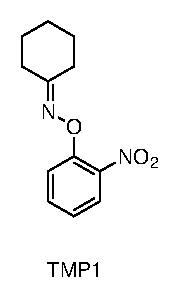
\includegraphics[scale=0.74]{Figures/cyclohexanone-oxime-2np.eps}
    \caption[\refcmpd{cyclohexanone-oxime-2np}]{The structure of \refcmpd{cyclohexanone-oxime-2np} exhibits a torsion of the nitro group, suggesting the Ch-bond is too weak to overcome the exchange repulsion between the oxygens.}
    \label{fig:cyclohexanone-oxime-2np}
    \end{figure}
    
    With this encouraging result, we sought to switch the Ch-bond back on again by improving the donor ability of the \emph{o}-nitro group.
    This was accomplished by introducing an electron donating group at the 5 position of the ring, which has the effect of increasing electron density at the \emph{o}-nitro group while leaving the oxime relatively unchanged.
    Compounds \cmpd{cyclohexanone-oxime-2n-5nme2p,cyclohexanone-oxime-2n-5mp} were prepared, both of which had similar electronic properties (\cref{fig:cyclohexanone-oxime-2n-5nme2p} and \cref{fig:cyclohexanone-oxime-2n-5mp}).
    
    \begin{figure}
    \centering
    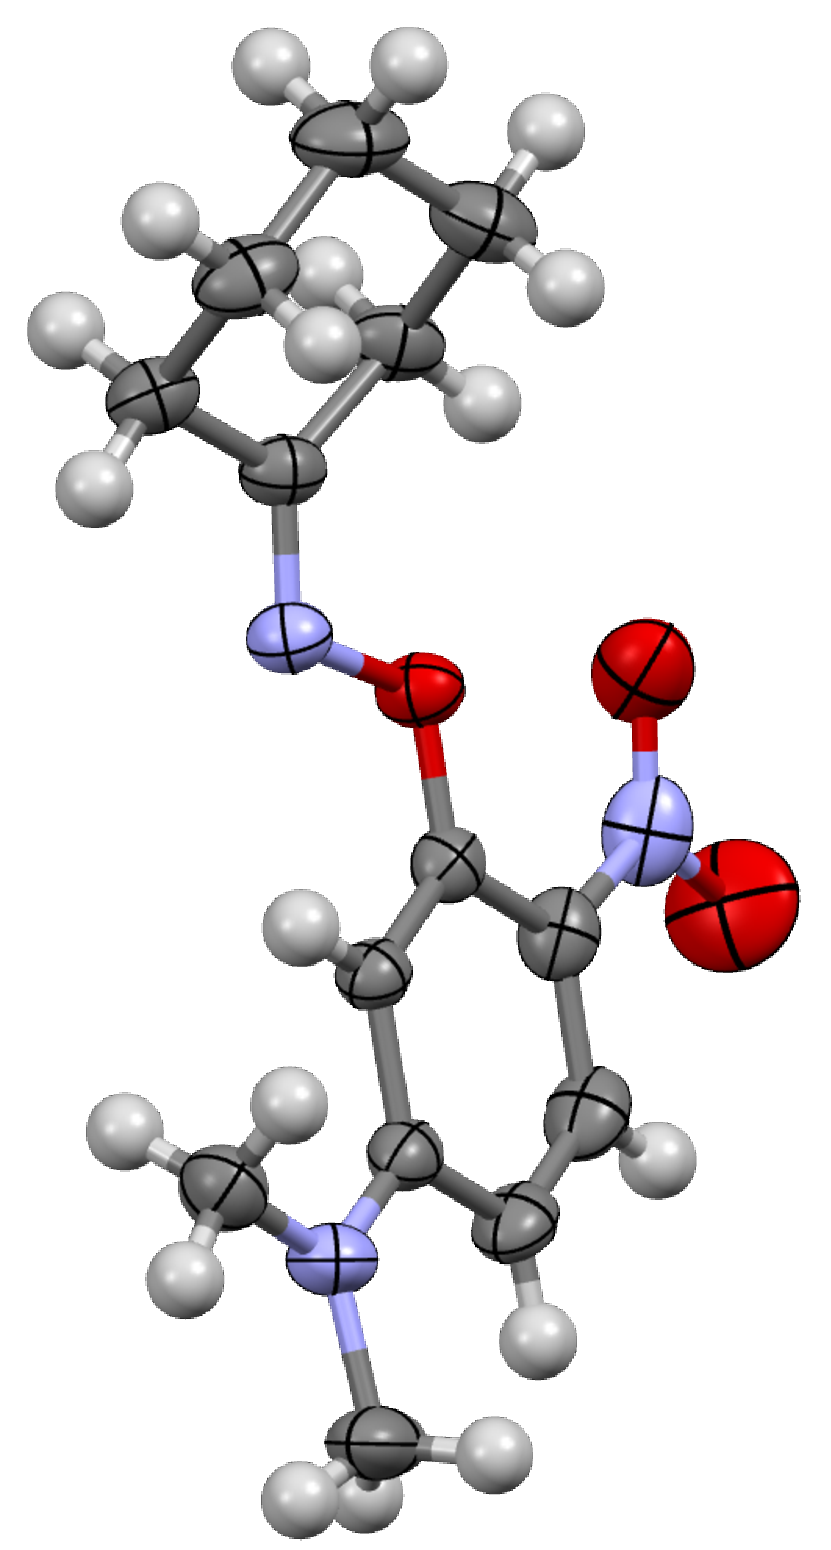
\includegraphics[height=4cm]{Figures/cyclohexanone-oxime-2n-5nme2p.pdf}
    \replacecmpd{cyclohexanone-oxime-2n-5nme2p}
    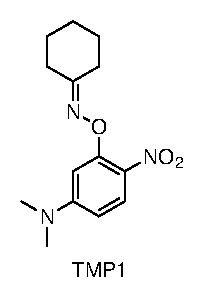
\includegraphics[scale=0.74]{Figures/cyclohexanone-oxime-2n-5nme2p.eps}
    \caption[\refcmpd{cyclohexanone-oxime-2n-5nme2p}]{The structure of \refcmpd{cyclohexanone-oxime-2n-5nme2p} features a coplanar nitro group. The increased basicity of the nitro oxygen is sufficient to overcome the repulsion.}
    \label{fig:cyclohexanone-oxime-2n-5nme2p}
    \end{figure}
    
    \begin{figure}
    \centering
    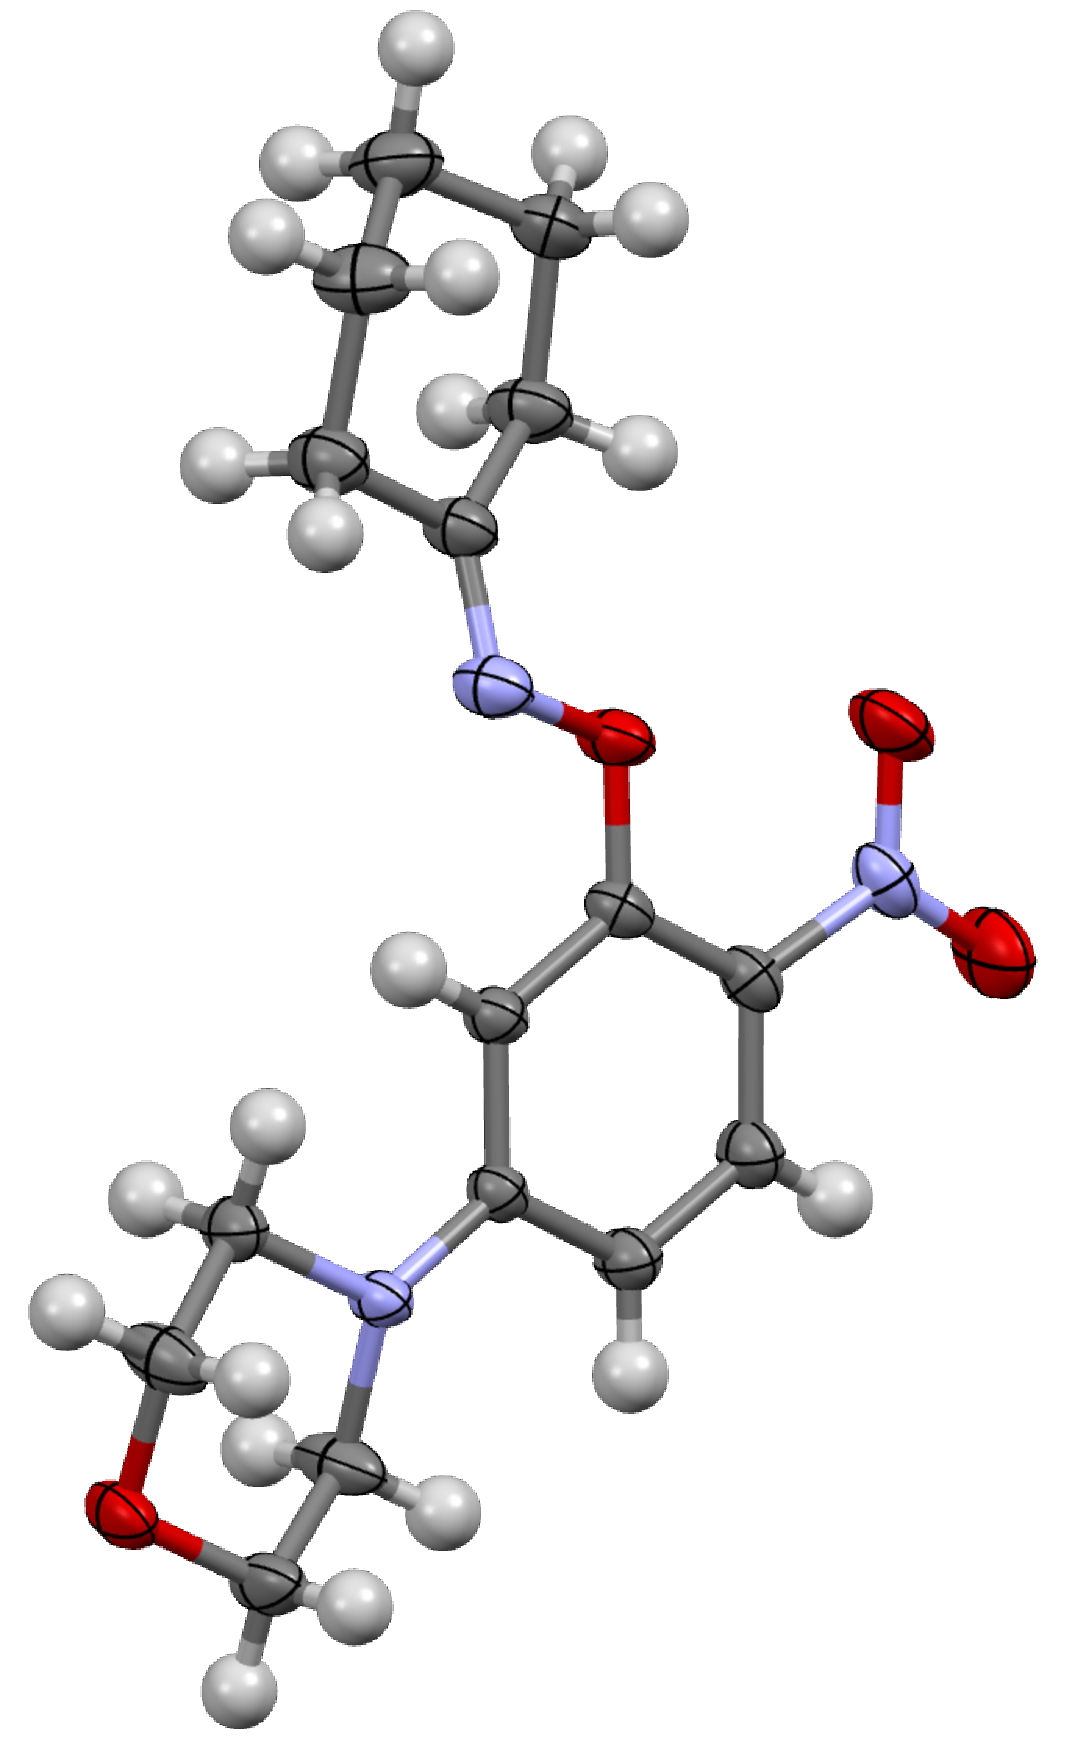
\includegraphics[height=4cm]{Figures/cyclohexanone-oxime-2n-5mpa.pdf}
    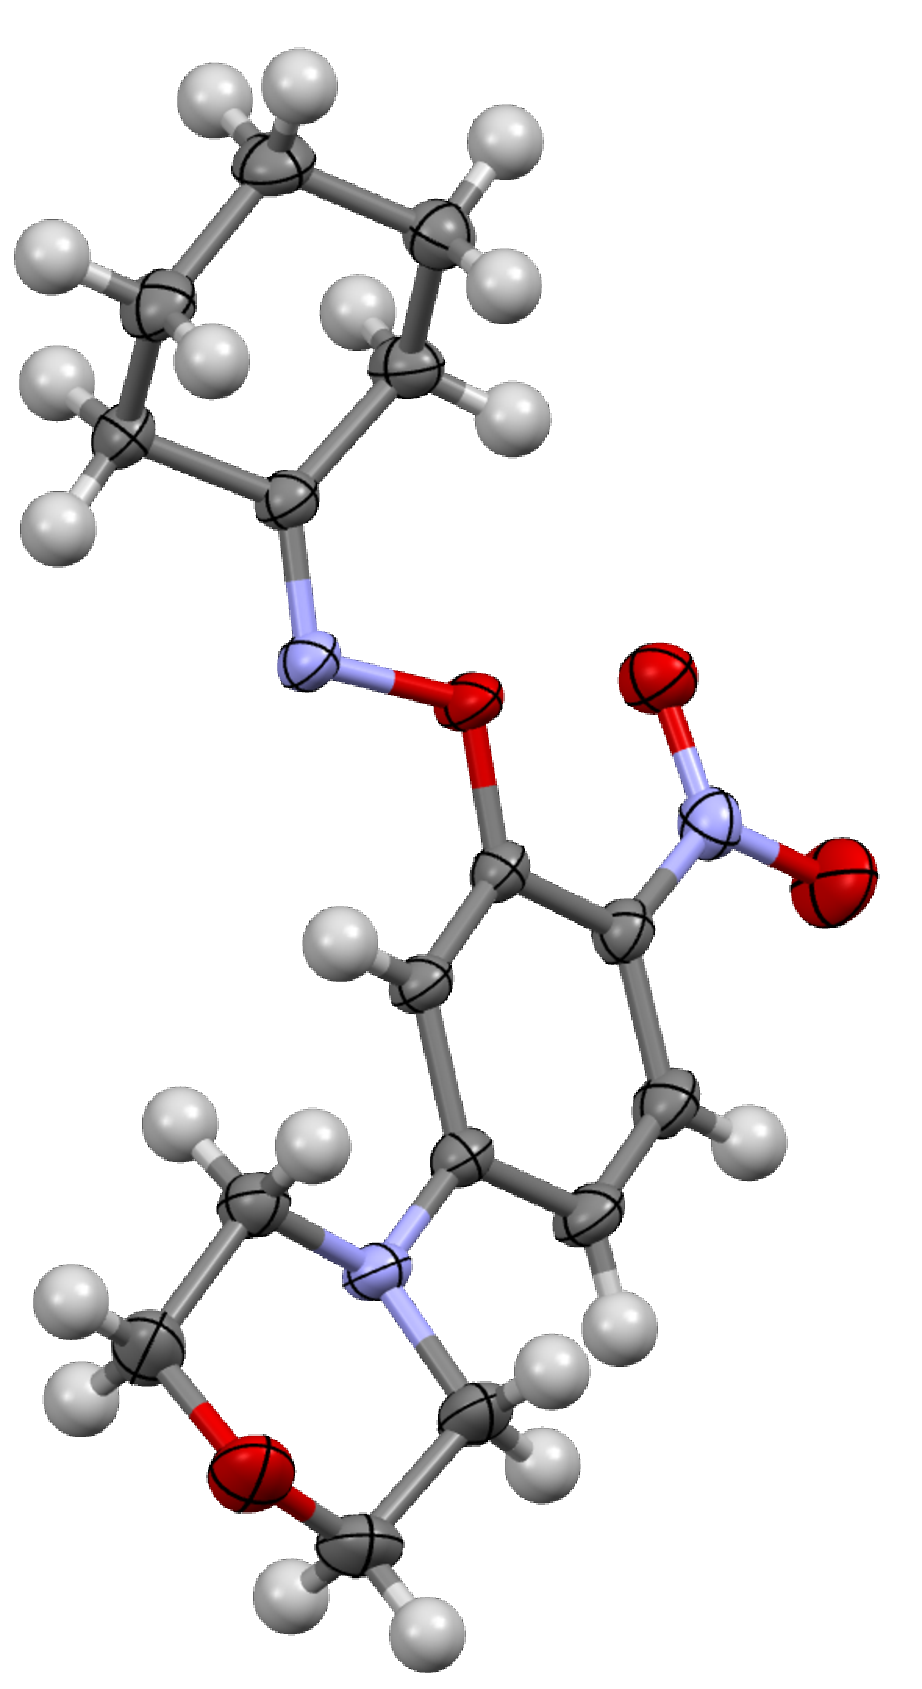
\includegraphics[height=4cm]{Figures/cyclohexanone-oxime-2n-5mpb.pdf}
    \replacecmpd{cyclohexanone-oxime-2n-5mp}
    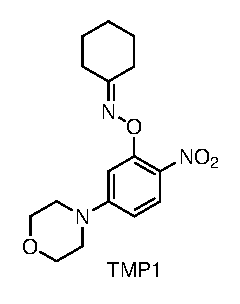
\includegraphics[scale=0.74]{Figures/cyclohexanone-oxime-2n-5mp.eps}
    \caption[\refcmpd{cyclohexanone-oxime-2n-5mp}]{The structure of \refcmpd{cyclohexanone-oxime-2n-5mp} also features coplanar nitro groups. There are two molecules in the asymmetric unit, and both are shown.}
    \label{fig:cyclohexanone-oxime-2n-5mp}
    \end{figure}
    
    \printbibliography
\end{refsection}

\begin{refsection}

    \chapter{Engineering supramolecular networks using Ch-bonding}
    
    \section{Introduction}
    
    \begin{figure}
        \replacecmpd{ebs.3py}
        \replacecmpd{ebs.3pyme}
        \replacecmpd{ebs.3pyhcl}
        \replacecmpd{selenylchloride-3py}
        \centering
        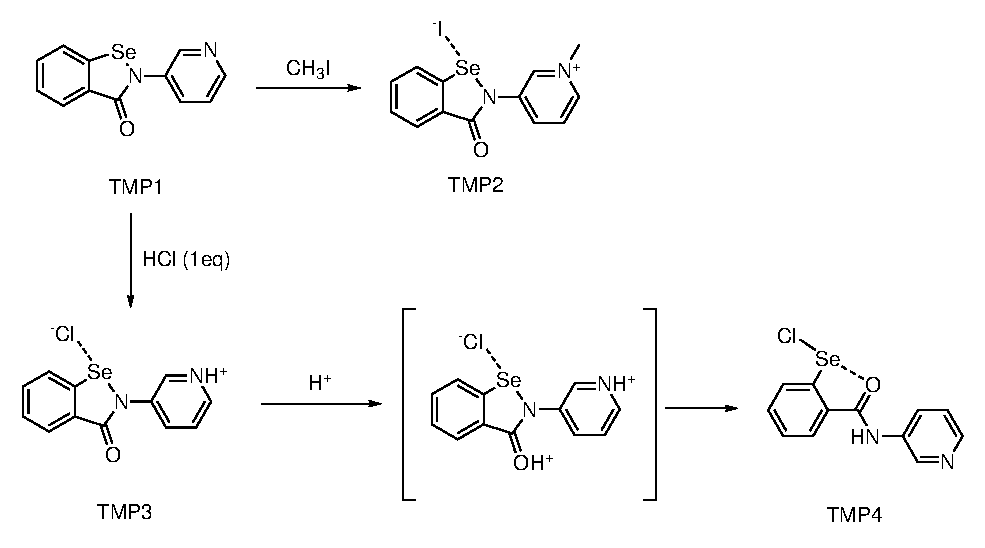
\includegraphics[scale=0.74]{Figures/ebs-3py-scheme.eps}
        \caption{Reactions of 3-pyridyl ebselen \refcmpd{ebs.3py}.}
        \label{sch:selenylchloride-mechanism}
    \end{figure}
    
    We prepared a 3-pyridyl ebselen derivative \cmpd{ebs.3py} in the hope that it would form a one-dimensional network consisting of linear Ch-bonded chains, and we were pleased to find that this was indeed the case.\autocite{???}
    
    In the crystal packing of \cmpd{ebs.3py}, each molecule is Ch-bonded through the pyridyl nitrogen to an adjacent molecule generated by the \textit{n}-glide, with a \ce{Se\dots N} distance of 2.386(1)~\AA.
    There is an additional Ch-bond to the carbonyl oxygen of the molecule generated by the \textit{n}-glide plus a translation along the \textit{a} axis (\cref{fig:3py-ebs-chbonds}).
    The \ce{Se\dots O} distance is 3.336(1)~\AA.
    The bond angles in both cases are consistent with a Ch-bonding interaction, with the nitrogen and oxygen atoms sitting almost perfectly opposite to the electron withdrawing group (174.43(5)\degree~and 165.89(4)\degree~respectively.)
    The $sp^2$ lone pairs of the nitrogen and oxygen atoms are also well aligned, at angles of 120.60(9)\degree~and 113.93(9)\degree~respectively.
    
    \begin{figure}
        \centering
        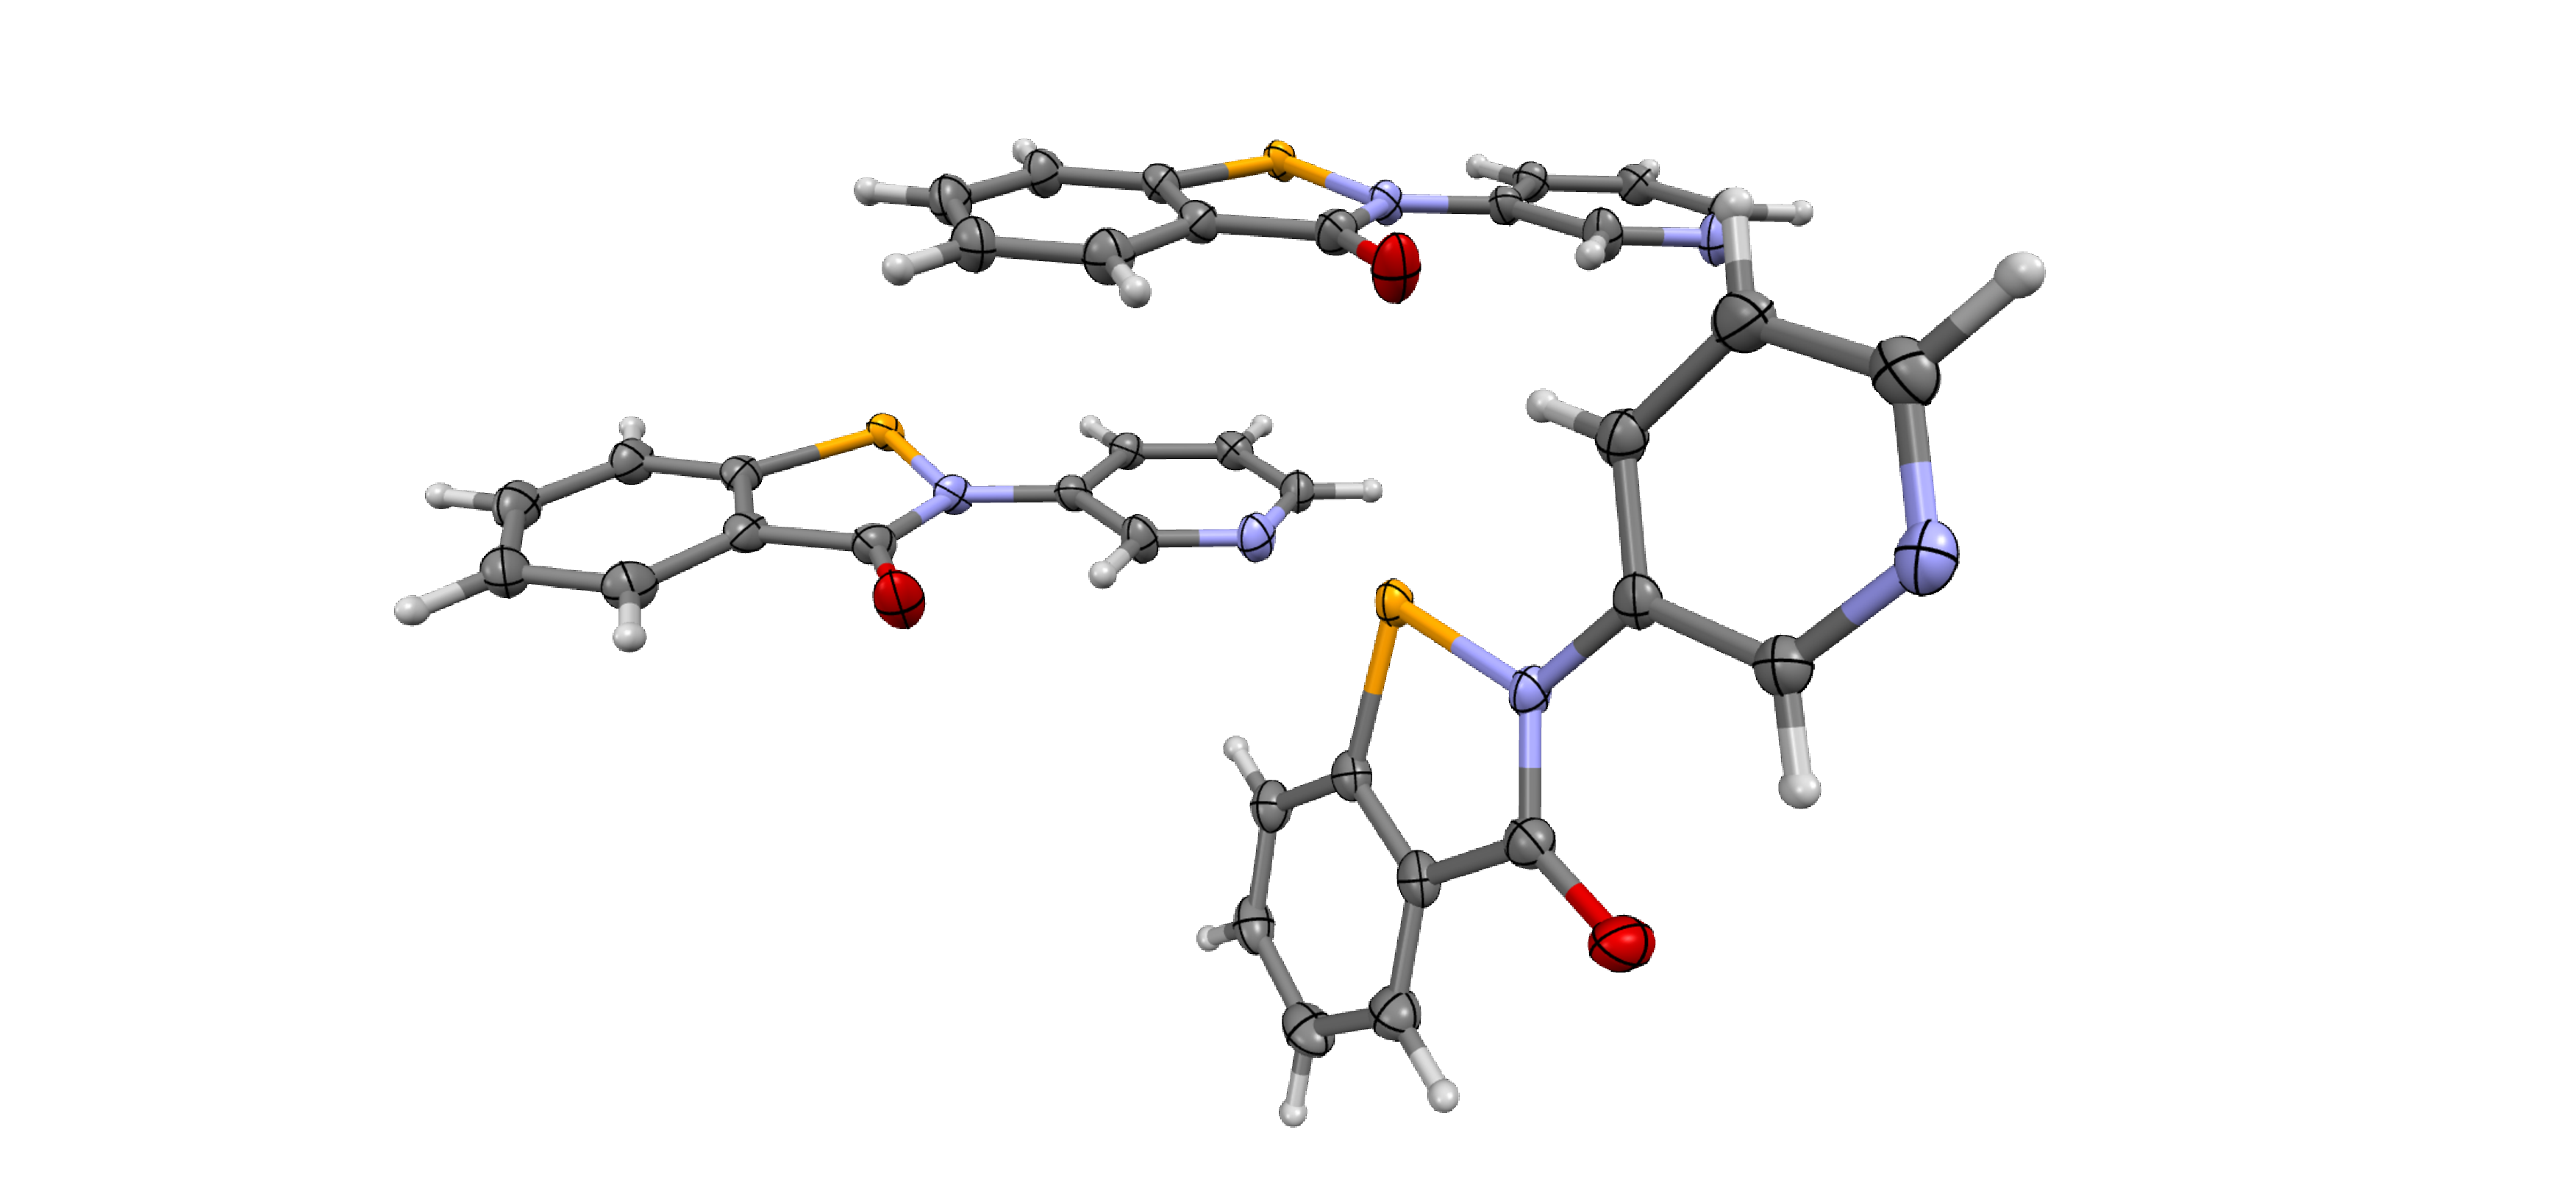
\includegraphics[width=\linewidth]{Figures/3py-ebs-chbonds.pdf}
        \caption{Ch-bonds formed by 3-pyridyl ebselen \refcmpd{ebs.3py} in the crystal packing. The stronger of the two is defined by the \ce{N-Se\cdots N_{pyr}} angle, and the weaker is defined by the \ce{C-Se\cdots O} angle.}
        \label{fig:3py-ebs-chbonds}
    \end{figure}
    
    \begin{figure}
        \centering
        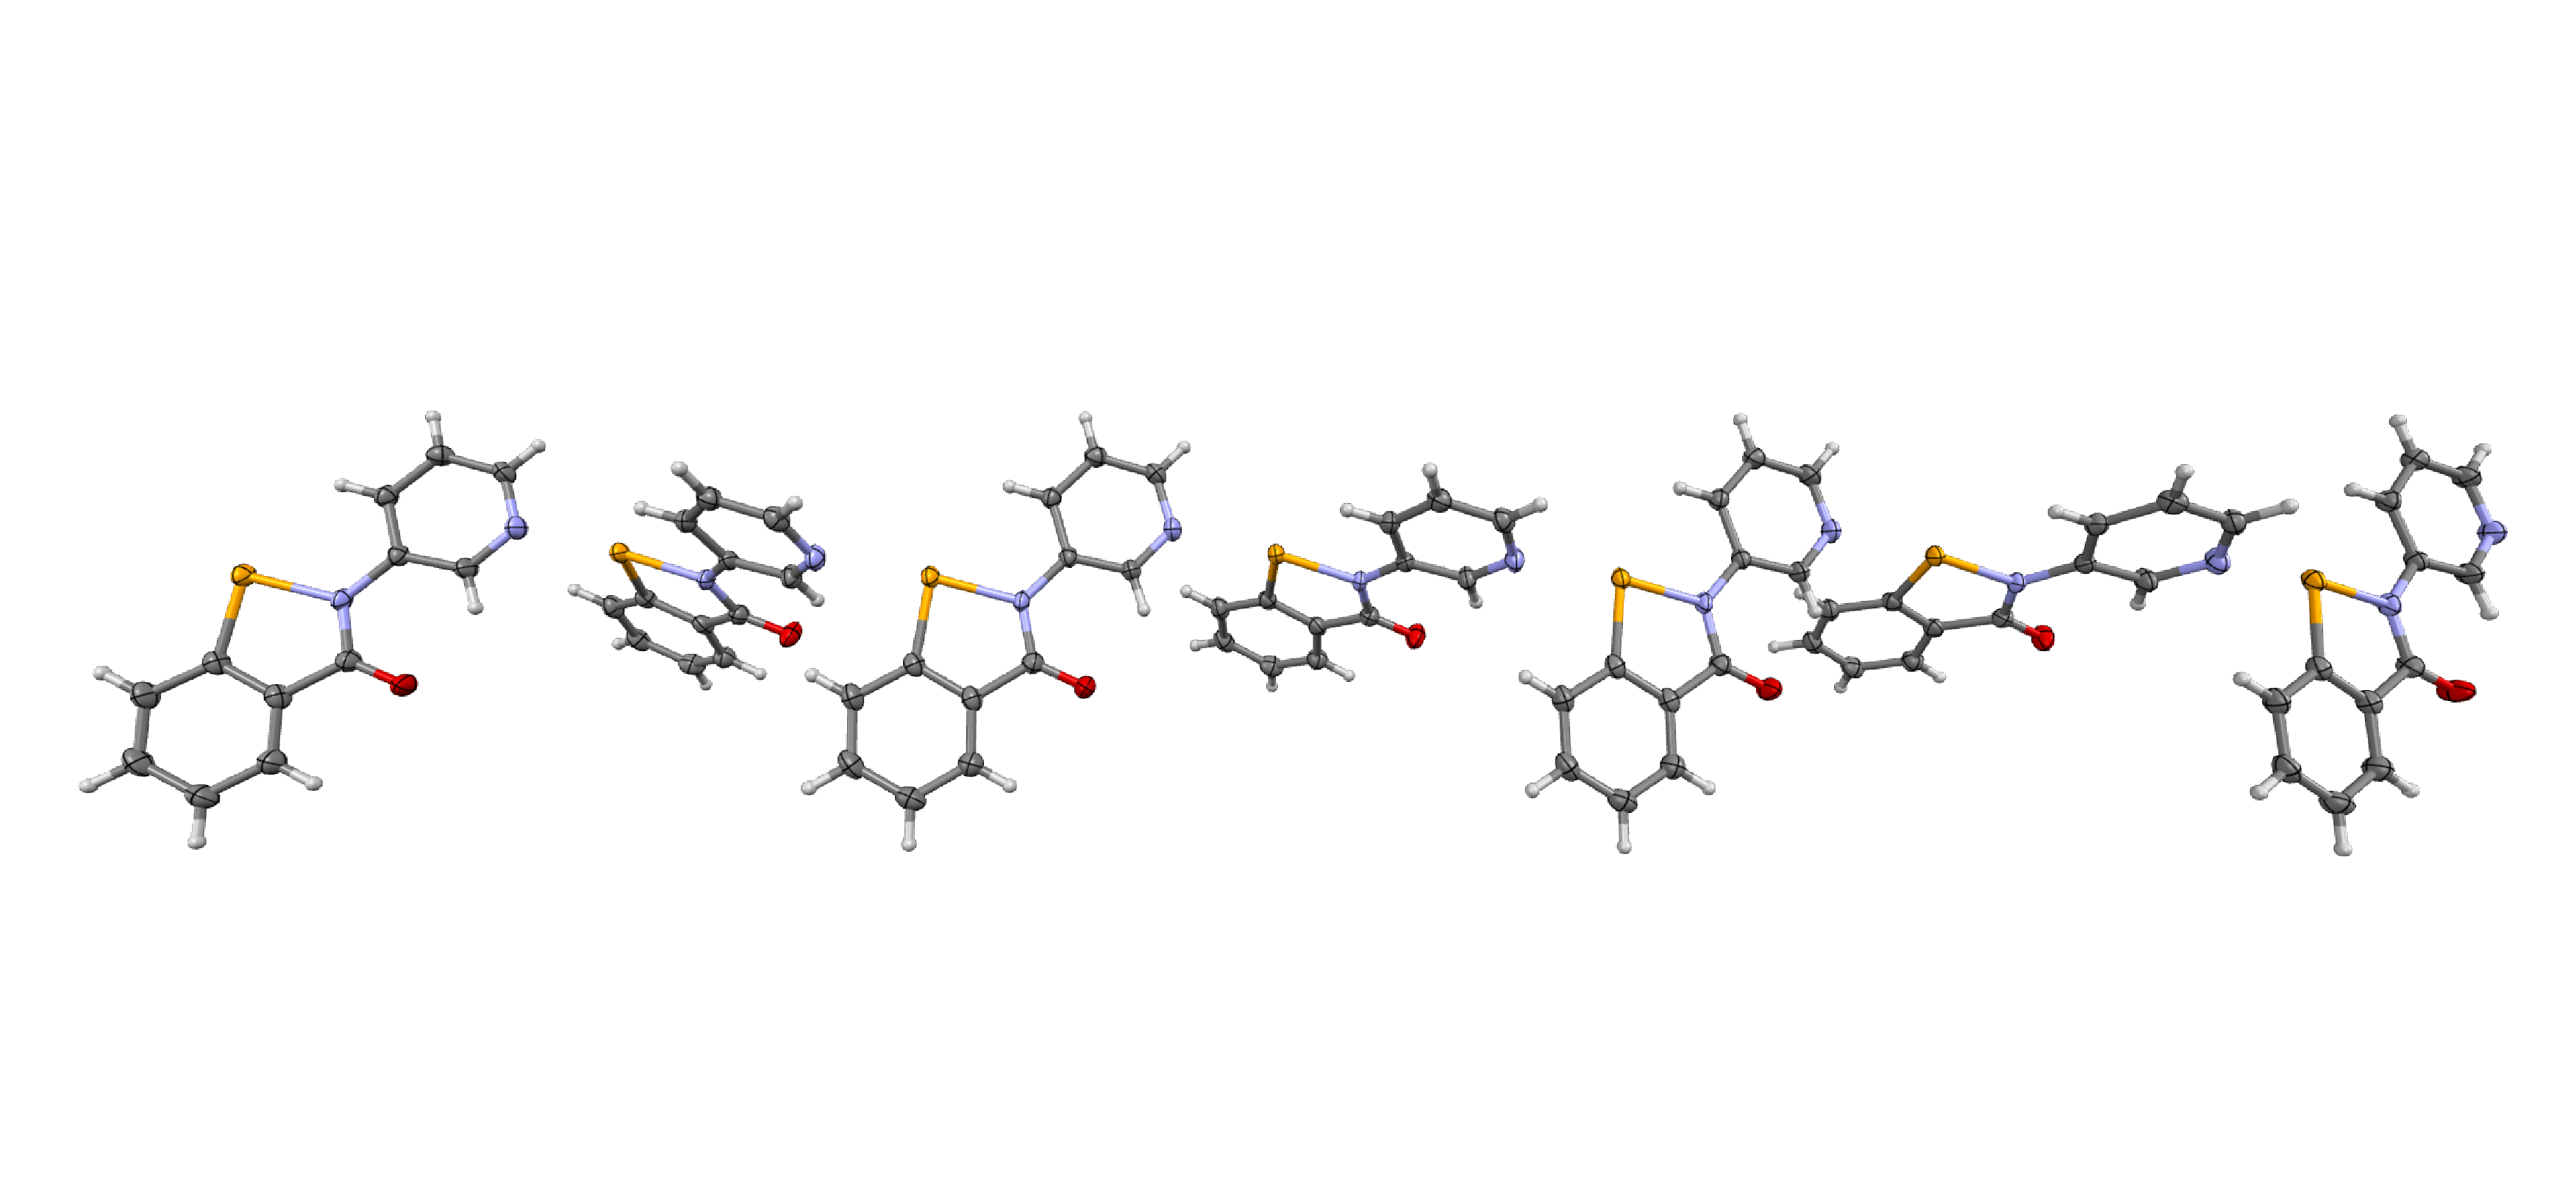
\includegraphics[width=\linewidth]{Figures/3py-ebs-chain.pdf}
        \caption{One-dimensional network formed by the strong \ce{N-Se\dots N} Ch-bonds. This is extended into 3 dimensions by the weaker \ce{C-Se\dots O} Ch-bonds, and $\pi$-stacking.}
        \label{fig:3py-ebs-chain}
    \end{figure}
    
    We have previously reported an instance of H-bond assisted Ch-bonding, in which a H-bond to the carbonyl of ebselen strengthens the resulting Ch-bond.
    We were interested to see if the introduction of a full positive charge in the molecule would have a similar effect, by analogy with charge-assisted H- and X-bonding.
    We therefore alkylated \cmpd{ebs.3py} using methyl iodide to form \cmpd{ebs.3pyme}, and were pleased to see yellow needles form in the reaction mixture almost immediately upon cooling.
    The structure of these crystals is shown in \cref{fig:3py-ebs-mei}.
    The pyridyl nitrogen is alkylated as expected, and the charge is balanced by the iodide Ch-bonded to the selenium, at a distance of 2.9904(4)~\AA~and an angle of 178.7(1)\degree~to the antipodal nitrogen.
    
    \begin{figure}
        \centering
        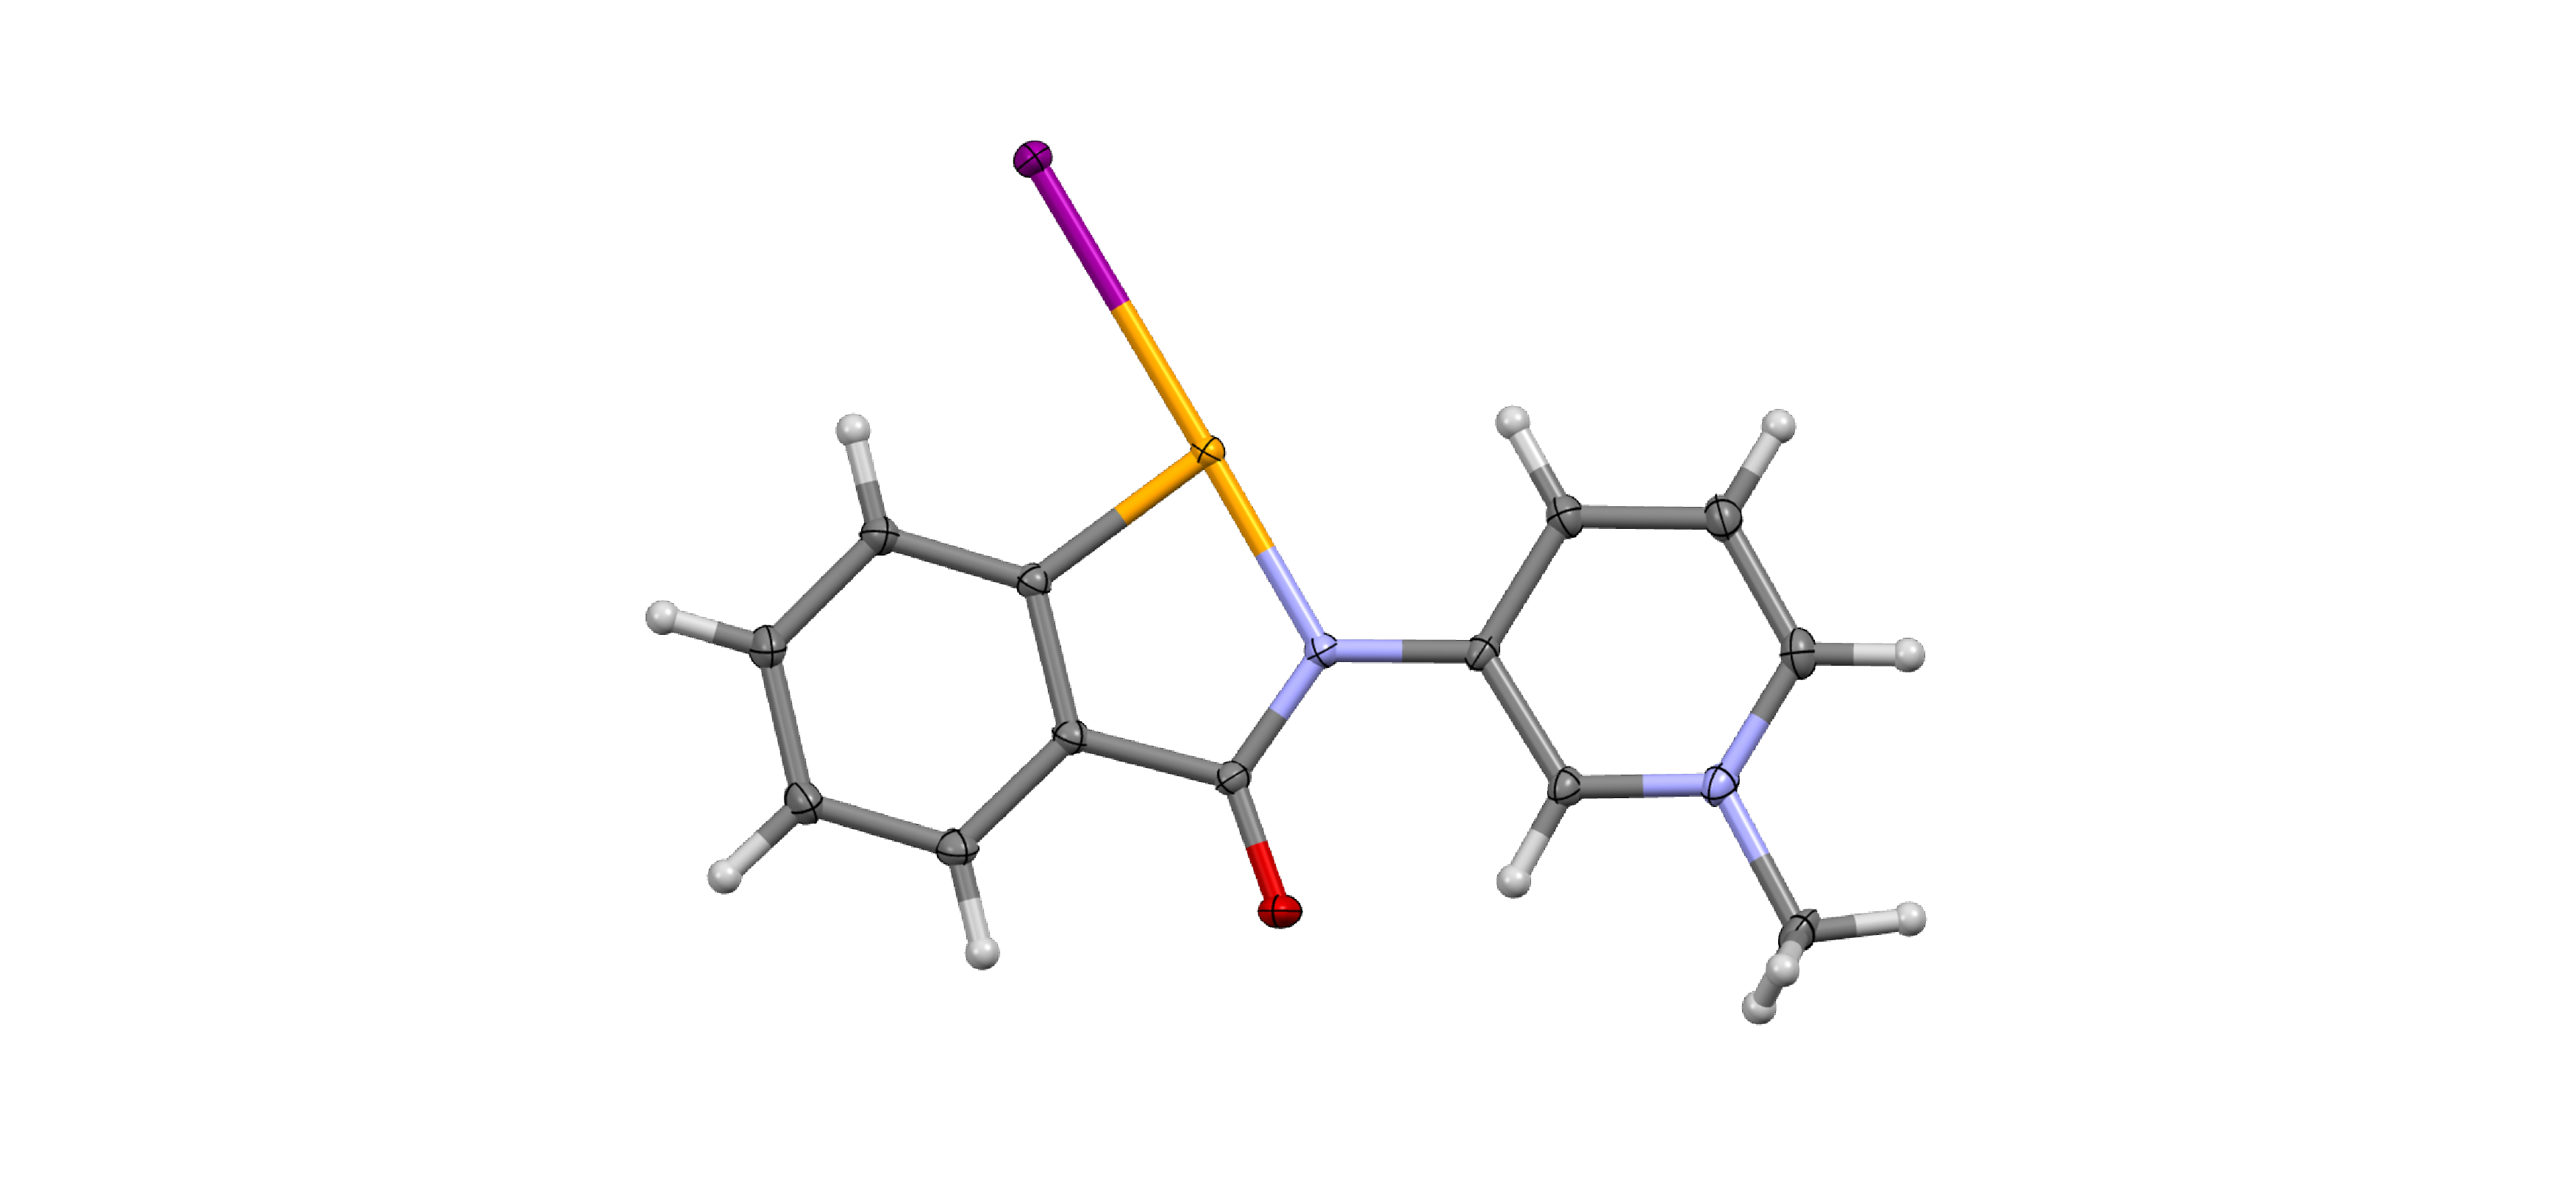
\includegraphics[width=\linewidth]{Figures/3py-ebs-mei.pdf}
        \caption{Structure of the methylated derivative \refcmpd{ebs.3pyme}.}
        \label{fig:3py-ebs-mei}
    \end{figure}
    
    In order to assess the effect of the positive charge on the Ch-bond, we required a system which lacked the charge on the ebselen molecule.
    We attempted to co-crystallise \cmpd{ebs.3py} with a variety of halide salts, but none gave the desired co-crystal.
    This is not entirely unsurprising, as most cations would not be easily incorporated in the lattice, disfavouring the formation of a co-crystal.
    However, when \cmpd{ebs.3py} was heated in aqueous \ce{HCl}, then slowly cooled, crystals of \cmpd{selenylchloride-3py} precipitated out of the solution (\cref{fig:3py-ebs-hcl}).
    The product \cmpd{selenylchloride-3py} corresponds to an extreme case of charge assisted Ch-bonding, where the endocyclic \ce{Se-N} bond is formally broken, and a new bond is established with the Ch-bond donor.
    We propose a mechanism for this transformation which involves protonation of the carbonyl oxygen by the strong acid, followed by nucleophilic attack by chloride at the selenium.
    The product then tautomerises to the more stable amide form, and an intramolecular Ch-bond is re-established, thus stabilising the selenyl chloride (\cref{sch:selenylchloride-mechanism}).
    The stability of this selenyl chloride is remarkable, as it is resistant to hydrolysis and oxidation, and may be kept in air for several weeks.
    
    \begin{figure}
        \centering
        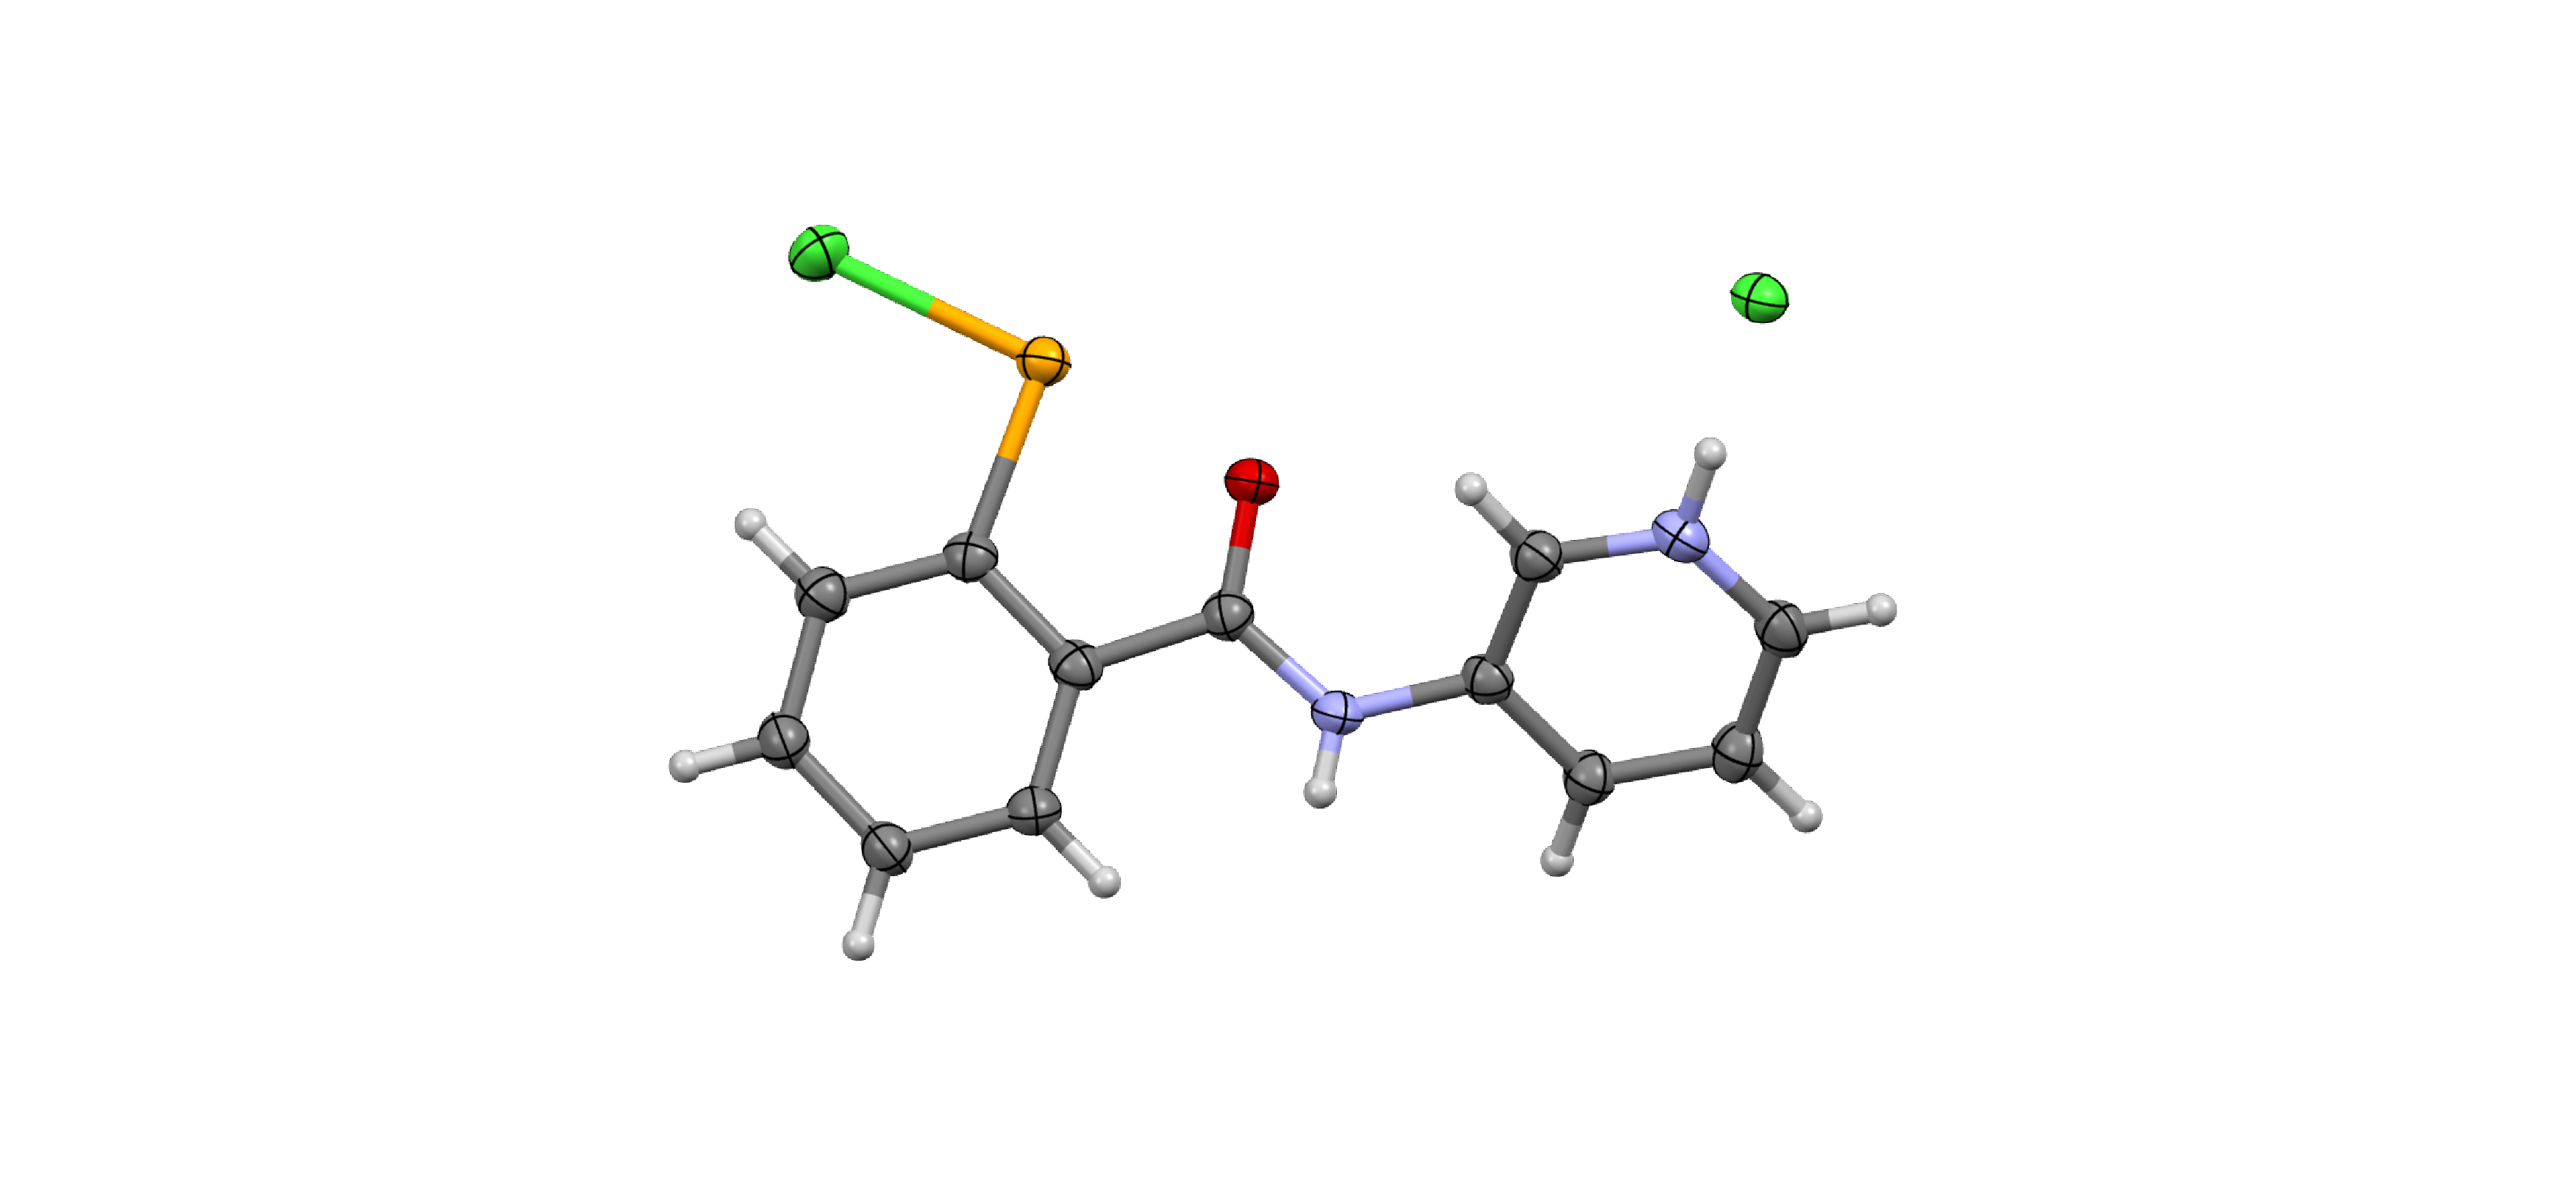
\includegraphics[width=\linewidth]{Figures/3py-ebs-hcl.pdf}
        \caption{Structure of the ring opened hydrochloride derivative \refcmpd{selenylchloride-3py}.}
        \label{fig:3py-ebs-hcl}
    \end{figure}
    
    \printbibliography[heading=subbibliography]
    
\end{refsection}